\documentclass[landscape]{article}
\pagenumbering{gobble}

\usepackage[a4paper]{geometry}
\usepackage[utf8]{inputenc}
\usepackage{tikz}
\usepackage[compat=1.1.0]{tikz-feynman}
\usepackage{graphicx}

\begin{document}
\centering
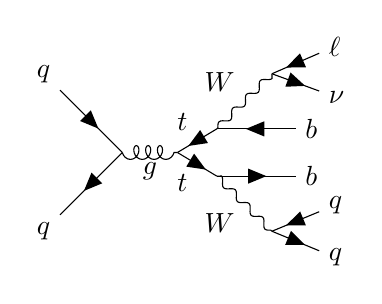
\begin{tikzpicture}
  \begin{feynman}
    % initial state particles
    \vertex (i1) {\(q\)};
    \vertex [below=2cm of i1] (i2) {\(q\)};

    % vertices
    \vertex [below right=1.cm and 1cm of i1] (a);
    \vertex [right=0.7cm of a] (b);

    % final state particles
    \vertex [above right=0.3cm and 0.5cm of b] (t1);
    \vertex [below right=0.3cm and 0.5cm of b] (t2);

    \vertex [above right=0.7cm and 0.7cm of t1] (W1);
    \vertex [right=1.0cm of t1] (f1) {\(b\)};

    \vertex [right=1.0cm of t2] (f2) {\(b\)};
    \vertex [below right=0.7cm and 0.7cm of t2] (W2);

    \vertex [above right=0.1cm and .6cm of W1] (f3) {\(\ell\)};
    \vertex [below right=0.1cm and .6cm of W1] (f4) {\(\nu\)};
    \vertex [above right=0.1cm and .6cm of W2] (f5) {\(q\)};
    \vertex [below right=0.1cm and .6cm of W2] (f6) {\(q\)};

    \diagram* {
      (i1) -- [fermion] (a)
        -- [fermion] (i2),

      (a) -- [gluon, edge label'=\(g\)] (b),

      (t1) -- [fermion, edge label'=\(t\)] (b)
        -- [fermion, edge label'=\(t\)] (t2),

      (f1) -- [fermion] (t1)
        -- [boson, edge label=\(W\)] (W1),
      (W2) -- [boson, edge label=\(W\)] (t2)
       -- [fermion] (f2),

      (f3) -- [fermion] (W1)
        -- [fermion] (f4),
      (f5) -- [fermion] (W2)
        -- [fermion] (f6),
    };


  \end{feynman}
\end{tikzpicture}%
\end{document}
